%===============================================================================
% LaTeX sjabloon voor de bachelorproef toegepaste informatica aan HOGENT
% Meer info op https://github.com/HoGentTIN/latex-hogent-report
%===============================================================================

\documentclass[dutch,dit,thesis]{hogentreport}

% TODO:
% - If necessary, replace the option `dit`' with your own department!
%   Valid entries are dbo, dbt, dgz, dit, dlo, dog, dsa, soa
% - If you write your thesis in English (remark: only possible after getting
%   explicit approval!), remove the option "dutch," or replace with "english".

\usepackage{pdfpages}

%% Pictures to include in the text can be put in the graphics/ folder
\graphicspath{{../graphics/}}

%% For source code highlighting, requires pygments to be installed
%% Compile with the -shell-escape flag!
\usepackage[chapter]{minted}
%% If you compile with the make_thesis.{bat,sh} script, use the following
%% import instead:
%% \usepackage[chapter,outputdir=../output]{minted}
\usemintedstyle{solarized-light}

%% Formatting for minted environments.
\setminted{%
    autogobble,
    frame=lines,
    breaklines,
    linenos,
    tabsize=4
}

% Other packages not already included can be imported here

%%---------- Document metadata -------------------------------------------------
% TODO: Replace this with your own information
\author{Torben de Schrijver}
\supervisor{Dhr. J. Claes}
\cosupervisor{Dhr. N. Nelissen}
\title{Mens versus model: Analyse van bepalende factoren en interpreteerbare machine-learningvoorspellingen van wedstrijdstatistieken in de Jupiler Pro League}
\academicyear{\advance\year by -1 \the\year--\advance\year by 1 \the\year}
\examperiod{1}
\degreesought{\IfLanguageName{dutch}{Professionele bachelor in de toegepaste informatica}{Bachelor of applied computer science}}
\partialthesis{false} %% To display 'in partial fulfilment'
%\institution{Internshipcompany BVBA.}

%% Add global exceptions to the hyphenation here
\hyphenation{back-slash}

%% The bibliography (style and settings are  found in hogentthesis.cls)
\addbibresource{bachproef.bib}            %% Bibliography file
\addbibresource{../voorstel/voorstel.bib} %% Bibliography research proposal
\defbibheading{bibempty}{}

%% Prevent empty pages for right-handed chapter starts in twoside mode
\renewcommand{\cleardoublepage}{\clearpage}

\renewcommand{\arraystretch}{1.2}

%% Content starts here.
\begin{document}

%---------- Front matter -------------------------------------------------------

\frontmatter

\hypersetup{pageanchor=false} %% Disable page numbering references
%% Render a Dutch outer title page if the main language is English
\IfLanguageName{english}{%
    %% If necessary, information can be changed here
    \degreesought{Professionele Bachelor toegepaste informatica}%
    \begin{otherlanguage}{dutch}%
       \maketitle%
    \end{otherlanguage}%
}{}

%% Generates title page content
\maketitle
\hypersetup{pageanchor=true}

%%=============================================================================
%% Voorwoord
%%=============================================================================

\chapter*{\IfLanguageName{dutch}{Woord vooraf}{Preface}}%
\label{ch:voorwoord}

Deze bachelorproef vormt het sluitstuk van mijn opleiding Toegepaste Informatica aan HOGENT. 
Tijdens het uitvoeren van dit onderzoek kreeg ik de kans om mijn interesse in voetbal, 
data-analyse en machine learning te combineren in een onderwerp dat zowel technisch als inhoudelijk uitdagend was. 
Het proces bracht niet alleen nieuwe inzichten met zich mee op vlak van data-analyse en modelontwikkeling, 
maar leerde mij ook kritisch omgaan met onderzoeksresultaten en wetenschappelijke methodologie.

\vspace{5pt}

Graag wil ik in het bijzonder mijn promotor, Dhr. J. Claes, bedanken voor de begeleiding gedurende dit traject. 
Zijn feedback rond de structuur van de bachelorproef, de uitwerking van grafieken en 
de tussentijdse evaluaties heeft een belangrijke bijdrage geleverd aan de kwaliteit van dit werk.

\vspace{5pt}

Daarnaast wil ik ook mijn co-promotor, Dhr. N. Nelissen, bedanken voor de tijd die hij vrijmaakte voor overlegmomenten en 
het beantwoorden van technische vragen tijdens het onderzoek.
%%=============================================================================
%% Samenvatting
%%=============================================================================

\chapter*{\IfLanguageName{dutch}{Samenvatting}{Abstract}}

Voetbalanalyse maakt steeds vaker gebruik van data-gedreven methoden,
maar de verklaringen die hieruit voortvloeien worden zelden systematisch vergeleken met de intuïtie van menselijke experts.
Deze bachelorproef onderzoekt welke factoren bepalend zijn voor wedstrijdstatistieken in de Jupiler Pro League
en stelt de vraag in welke mate interpreteerbare machine-learningmodellen en voetbalexperts overeenstemmen
in hun voorspellingen en verklaringen.

\vspace{5pt}

Het onderzoek vertrekt vanuit een dataset van 2006 wedstrijden uit de Jupiler Pro League, verzameld over de seizoenen 2019-2020
tot en met 2025-2026. Naast de wedstrijdstatistieken werden ook externe factoren opgenomen,
waaronder weergegevens (temperatuur, neerslag, windsnelheid) en stadioninformatie.
Op basis van deze ruwe data werden via feature engineering nieuwe variabelen gecreëerd,
zoals een dynamische rangschikking, recente vorm, head-to-head statistieken, een speelstijlscore
en indicatoren voor titel- en degradatiewedstrijden. Alle data werden opgeslagen in een relationele databank.

\vspace{5pt}

Het onderzoek verliep in vijf fasen: dataverzameling en voorbereiding, feature engineering,
exploratieve en statistische analyse, modelontwikkeling en evaluatie, en modelinterpretatie en vergelijking.
Voor de analyse van het wedstrijdresultaat werden vier interpreteerbare classificatiemodellen vergeleken:
Logistic Regression, Random Forest, Gradient Boosting en XGBoost.
Aanvullend werden voor het aantal schoten, doelpunten en kaarten XGBoost-regressiemodellen ontwikkeld.
Feature importance en SHAP-waarden werden gebruikt om de modellen te interpreteren.
Parallel hiermee werden zes voetbalexperts met een professionele achtergrond in het Belgische voetbal en de sportjournalistiek bevraagd via een enquête.

\vspace{5pt}

De resultaten tonen aan dat recente vorm en rangverschil de meest bepalende
voorspellers zijn voor het wedstrijdresultaat. Het thuisvoordeel is statistisch aantoonbaar
(43,28\% thuisoverwinningen tegenover 32,37\% voor de bezoeker), maar beperkt in relatief belang.
Onderlinge confrontaties (H2H) zijn statistisch significant maar zwak als enige voorspeller.
Het beste classificatiemodel, Logistic Regression, behaalde een accuraatheid van 55,97\%,
in lijn met wat in de internationale literatuur gerapporteerd wordt voor voetbalvoorspellingen.

\vspace{5pt}

Voor doelpunten bleek de speelstijlcombinatie aanvallend versus verdedigend de enige statistisch significant
beïnvloedende factor (p = 0,0139). Voor kaarten werden enkel degradatiewedstrijden als significant bevonden (p = 0,0399).
Het aantal schoten bleef het moeilijkst te modelleren, met een negatieve R²-waarde, 
wat aangeeft dat het verloop van een wedstrijd sterk door toeval wordt bepaald of er niet de geschikte data gebruikt werd.

\vspace{5pt}

De vergelijking tussen model en experts toont een gedeeltelijke overeenstemming.
Beide benaderingen identificeren recente vorm en rangverschil als de voornaamste factoren voor het wedstrijdresultaat,
en erkennen speelstijl als relevant voor doelpunten en kaarten.
Tegelijk zijn er duidelijke verschillen: experts overschatten de voorspellende waarde van H2H-resultaten en derby's,
terwijl de modellen gevoelig zijn voor temperatuur als seizoensgerelateerde externe variabele.

\vspace{5pt}

Dit onderzoek draagt bij aan de sportanalytics door historische data, 
interpreteerbare modellen en menselijke expertise samen te onderzoeken binnen de context van de Jupiler Pro League.
De bevindingen zijn nuttig voor clubs, analisten en journalisten die datagedreven inzichten willen integreren in hun
besluitvorming. Toekomstig onderzoek kan worden versterkt door het opnemen van scheidsrechtersdata,
individuele spelersinformatie en een grotere expertsteekproef.


%---------- Inhoud, lijst figuren, ... -----------------------------------------

\tableofcontents

% In a list of figures, the complete caption will be included. To prevent this,
% ALWAYS add a short description in the caption!
%
%  \caption[short description]{elaborate description}
%
% If you do, only the short description will be used in the list of figures

\listoffigures

% If you included tables and/or source code listings, uncomment the appropriate
% lines.
\listoftables

% Als je een lijst van afkortingen of termen wil toevoegen, dan hoort die
% hier thuis. Gebruik bijvoorbeeld de ``glossaries'' package.
% https://www.overleaf.com/learn/latex/Glossaries

%---------- Kern ---------------------------------------------------------------

\mainmatter{}

% De eerste hoofdstukken van een bachelorproef zijn meestal een inleiding op
% het onderwerp, literatuurstudie en verantwoording methodologie.
% Aarzel niet om een meer beschrijvende titel aan deze hoofdstukken te geven of
% om bijvoorbeeld de inleiding en/of stand van zaken over meerdere hoofdstukken
% te verspreiden!

\input{inleiding}
\input{standvanzaken}
\input{methodologie}
\chapter{\IfLanguageName{dutch}{Dataverzameling en voorbereiding}{Data collection and preparation}}%
\label{ch:dataverzameling}

In dit hoofdstuk concentreren we ons op de gebruikte data en hoe deze verzameld en voorbereid zijn voor analyse.
Eerst wordt besproken waar de gegevens vandaan komen, hoe de dataset eruitziet en waarom deze gegevens waardevol zijn voor de bachelorproef.

\section{Dataverzameling}

Voordat de dataset verwerkt kan worden voor de modellen, moet deze eerst verzameld worden.
Daarom werd er vooraf grondig gezocht naar verschillende bronnen met bruikbare ruwe data,
die later tot een gestructureerd geheel konden worden gebracht.
Deze gegevens bestonden uit wedstrijdstatistieken van de Jupiler Pro League,
evenals externe factoren zoals weerdata en stadioninformatie. Nadien werden deze gestructureerd en opgeslagen in een relationele databank.

\subsection{Wedstrijddata}

Eerst werden 7 CSV-bestanden gedownload~\autocite{football_data_belgium}.
Elk bestand bevatte een bepaald seizoen van de Jupiler Pro League, beginnend bij het seizoen 2019-2020 en eindigend vóór de play-offs van het seizoen 2025-2026.
Voorgaande seizoenen werden niet opgenomen omdat er in deze bestanden bepaalde statistieken ontbraken die van belang waren.
Uit deze bron werden diverse wedstrijdstatistieken verzameld,
waaronder de deelnemende teams, de speeldatum en de uiteindelijke winnaar.
Daarnaast werden ook het aantal doelpunten, schoten, overtredingen, corners en kaarten voor zowel de thuis- als uitploeg verzameld.
Voor de feature importance-analyse en de voorspellingen waren deze variabelen uiteraard cruciaal.
Variabelen zoals betting odds werden bewust niet opgenomen omdat deze juist voorspeld moesten worden.
Overige data van de scheidsrechter, teamopstellingen, blessures en transfers waren enkel beschikbaar via betaalde bronnen en werden daarom niet opgenomen.

\subsection{Externe factoren}

Eveneens werden externe factoren toegevoegd aan de dataset.
Hiertoe behoren onder andere weergegevens zoals temperatuur, neerslag, luchtvochtigheid, windsnelheid, bewolking, weercode en luchtdruk.
Deze variabelen werden per uur opgehaald via de API van~\textcite{open_meteo_api}.
Ook deze gegevens waren van belang omdat ze mogelijk een invloed konden hebben op de wedstrijdstatistieken en dus ook op de voorspellingen.

\vspace{5pt}

Aanvullend werden de coördinaten van de verschillende stadions opgezocht. Deze waren vereist als parameters voor het ophalen van de weerdata.
Naast de ligging van het stadion werd ook de stadioncapaciteit opgenomen als feature. 
Hoewel deze variabele geen exacte maat vormt voor het effectieve aantal aanwezige toeschouwers, kan ze wel dienen als een benadering van de schaal van het thuispubliek en de infrastructuur van de club. 
Zo kon onderzocht worden of stadiongrootte en het aantal supporters, met merendeels steun voor de thuisploeg, samenhangt met bepaalde wedstrijdstatistieken.

\subsection{Dataopslag}

Na het verzamelen van de verschillende gegevens werden deze gestructureerd en opgeslagen in een relationele databank om consistentie en toegankelijkheid te garanderen.
Deze databank werd beheerd met behulp van Microsoft SQL Server in SQL Server Management Studio (SSMS).
Figuur \ref{fig:databank-schema} toont de structuur van de databank met de verschillende tabellen en relaties.

\begin{figure}[h!]
\centering
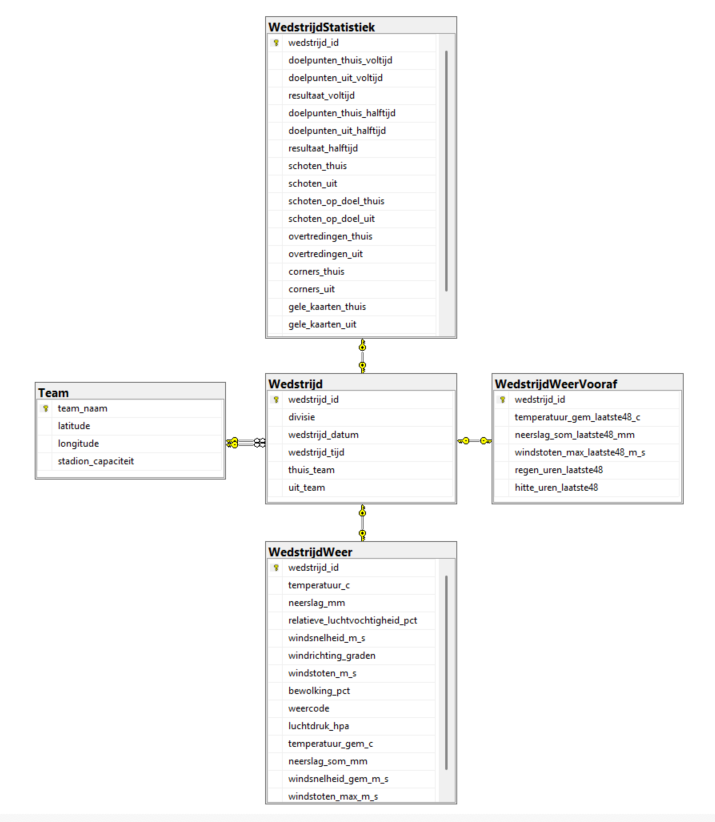
\includegraphics[width=0.8\textwidth]{databank_schema.png}
\caption{Schematische weergave van de relationele databank}
\label{fig:databank-schema}
\end{figure}

\vspace{5pt}

Hierin werd alle data van de wedstrijdstatistieken in de tabel \textit{WedstrijdStatistiek} opgeslagen.
Deze tabel verwees naar de tabel \textit{Wedstrijd}, waarin de details van elke wedstrijd werden bijgehouden, zoals datum, tijd en teams.
Daarnaast was er nog een tabel \textit{Team}, die de locatie en capaciteit van elk stadion bevatte.
Overigens waren er nog twee tabellen voor de weerdata. De tabel \textit{WedstrijdWeer} bevatte de weersomstandigheden op het moment van de aftrap. 
Omdat de API weergegevens per uur aanleverde, werd het uur van de wedstrijd als referentiepunt genomen. 
Daarnaast werden ook gemiddelden berekend binnen een tijdsvenster van één uur rond de aftrap om de weersomstandigheden tijdens de wedstrijd beter te benaderen.
De tabel \textit{WedstrijdWeerVooraf} bevatte weergegevens van de 48 uur voorafgaand aan de wedstrijd. 
Deze bevatten het gemiddelde van de temperatuur, de som van de hoeveelheid neerslag en de maximale windsnelheid.
\chapter{Feature Engineering}
\label{ch:feature-engineering}

In deze fase van het onderzoek werd feature engineering toegepast om op basis van ruwe wedstrijddata nieuwe, informatieve variabelen te construeren. 
Het doel van deze stap is het verhogen van de voorspellende kracht van de dataset en het toevoegen 
van contextuele en interpreteerbare informatie voor de machine learning-modellen. Alle dynamische features werden zodanig geconstrueerd 
dat uitsluitend gebruik werd gemaakt van historische informatie om datalekage te vermijden.

\vspace{5pt}

\subsection{Seizoensvariabele}

Elke wedstrijd werd toegewezen aan een specifiek seizoen op basis van de datum. 
Wedstrijden gespeeld tussen juli en december werden toegewezen aan het seizoen startjaar/startjaar+1, 
terwijl wedstrijden tussen januari en juni werden toegewezen aan het vorige startjaar/startjaar+1 seizoen. 
Deze variabele maakt het mogelijk om prestaties te groeperen binnen competitieve contexten.

\vspace{5pt}

\subsection{Dynamische rangschikking}

Voor elke wedstrijd werd een tussentijdse rangschikking berekend op basis van alle voorgaande wedstrijden binnen hetzelfde seizoen. 
Teams kregen 3 punten voor een overwinning, 1 punt voor een gelijkspel en 0 punten voor een nederlaag. 
Daarnaast werd het doelsaldo berekend als het verschil tussen gemaakte en geïncasseerde doelpunten.

De rangschikking werd dynamisch bepaald op elk wedstrijdmoment door teams te sorteren op:
\begin{itemize}
    \item totaal aantal punten (aflopend)
    \item doelsaldo (aflopend)
\end{itemize}

Deze aanpak simuleert de evolutie van de competitietabel doorheen het seizoen.

\vspace{5pt}

\subsection{Recente vorm}

De vorm van een team werd gedefinieerd als het gemiddelde aantal behaalde punten over de laatste vijf gespeelde wedstrijden vóór de betreffende wedstrijd. 
Elke wedstrijdresultaat werd omgezet naar een numerieke score (3 voor winst, 1 voor gelijkspel, 0 voor verlies). 

Formeel:

\[
\text{Form}_{t} = \frac{1}{5} \sum_{i=t-5}^{t-1} P_i
\]

waarbij $P_i$ het aantal behaalde punten in wedstrijd $i$ is.

Deze variabele geeft een indicatie van de recente prestatiecurve van een team en vangt tijdelijke fluctuaties in vorm op.

\vspace{5pt}

\subsection{Head-to-head statistieken}

Voor elke wedstrijd werden historische onderlinge confrontaties tussen beide teams geanalyseerd. 
Hierbij werd gekeken naar de laatste drie onderlinge wedstrijden vóór het huidige moment. De volgende variabelen werden berekend:

\begin{itemize}
    \item aantal overwinningen van het thuisteam
    \item aantal overwinningen van het uitteam
\end{itemize}

Op basis hiervan werd een binaire classificatie afgeleid die aangeeft welk team historisch voordeel heeft in de onderlinge duels.

\vspace{5pt}

\subsection{Titel- en degradatiewedstrijden}

Wedstrijden werden geclassificeerd als titelduels indien aan volgende voorwaarden werd voldaan:
\begin{itemize}
    \item beide teams staan in de top 2 van de rangschikking
    \item beide teams hebben meer dan 40 punten
    \item het puntenverschil bedraagt maximaal 5 punten
\end{itemize}

Degradatiewedstrijden werden gedefinieerd als wedstrijden die laat in het seizoen plaatsvinden waarbij 
beide teams zich in de onderste regionen van de rangschikking bevinden (laatste drie plaatsen) en het puntenverschil maximaal 3 punten bedraagt.

\vspace{5pt}

\subsection{Rivaliteitsindicator}

Op basis van vooraf gedefinieerde clubparen werd een binaire variabele toegevoegd die aangeeft of een wedstrijd een klassieke rivaliteit of derby betreft. 
Dit omvat onder andere regionale derby’s en historisch belangrijke confrontaties.

\vspace{5pt}

\subsection{Speelstijl van teams}

Voor elk team werd een speelstijlscore berekend op basis van geaggregeerde prestatie-indicatoren over de laatste vijf wedstrijden. 
Hierbij werden onder meer het aantal doelpunten, schoten en corners meegenomen.

De stijlscore werd gedefinieerd als:

\[
\text{Style Score} = (\text{doelpunten} + 0.3 \cdot \text{schoten}) - (\text{tegendoelpunten} + 0.3 \cdot \text{schoten tegen})
\]

Op basis van de verdeling van deze score werden teams ingedeeld in drie categorieën:
\begin{itemize}
    \item Aanvallend
    \item Gebalanceerd
    \item Verdedigend
\end{itemize}

De drempels werden bepaald op basis van de 33e en 66e percentielen.

\vspace{5pt}

\subsection{Contextuele variabelen}

Daarnaast werden verschillende contextuele features toegevoegd:

\begin{itemize}
    \item Weekdag en weekendindicator
    \item Avondwedstrijden (start ≥ 18:00)
    \item Weersomstandigheden (regen, harde regen, hoge temperatuur)
    \item Stadioncapaciteit (gecategoriseerd in klein, middel en groot via kwantielen)
\end{itemize}

\vspace{5pt}

\subsection{Relatieve verschillen}

Tot slot werden relatieve verschillen tussen teams berekend:

\begin{itemize}
    \item Rangverschil: verschil in positie op de dynamische ranglijst
    \item Vormverschil: verschil in recente vorm (5 wedstrijden)
\end{itemize}

Deze features laten toe om directe comparatieve sterkte tussen teams te modelleren.

\vspace{5pt}

Door deze combinatie van domeinkennis, statistische aggregatie en contextuele informatie werd een uitgebreide feature space gecreëerd. 
Deze verrijkte dataset vormt de input voor de verdere exploratieve en statische data-analyse en de machine learning-modellen.
\input{resultaten}
\input{discussie}
%%=============================================================================
%% Conclusie
%%=============================================================================

\chapter{Conclusie}%
\label{ch:conclusie}

In deze bachelorproef werd onderzocht welke factoren bepalend zijn voor wedstrijdstatistieken in de Jupiler Pro League,
en in welke mate data-gedreven machine-learningmodellen en menselijke voetbalexperts overeenstemmen in hun voorspellingen en verklaringen.
In dit afsluitende hoofdstuk worden de onderzoeksvragen beantwoord op basis van de gevonden resultaten,
wordt de wetenschappelijke bijdrage van het werk toegelicht, en worden enkele aanbevelingen voor toekomstig onderzoek geformuleerd.

\section{Antwoord op de onderzoeksvragen}

\subsection*{Deelvraag 1: Welke team- en wedstrijdgerelateerde factoren zijn geassocieerd met het wedstrijdresultaat?}

Uit de historische data-analyse blijkt dat recente vorm en rangverschil de sterkste statistisch significante
associaties vertonen met het wedstrijdresultaat. Het thuisvoordeel is eveneens duidelijk aanwezig: 43,28\% van
de wedstrijden wordt gewonnen door de thuisploeg, tegenover 32,37\% door de bezoeker. Bij een rangverschil
van tien plaatsen of meer wint de hoger gerangschikte ploeg in 78,9\% van de gevallen. Onderlinge confrontaties (H2H)
tonen wel een statistisch significante associatie, maar de praktische voorspellende waarde blijft beperkt (38,29\% nauwkeurigheid als enkel criterium).

\subsection*{Deelvraag 2: Welke factoren beïnvloeden het verloop van wedstrijdstatistieken zoals doelpunten, schoten en kaarten?}

Voor het aantal doelpunten is de speelstijlcombinatie aanvallend versus verdedigend de enige factor
met een statistisch significant effect (p = 0,0139). Wedstrijden in deze configuratie leveren gemiddeld 3,19 doelpunten op,
tegenover een algemeen gemiddelde van 2,86. Het model voor doelpunten bevestigt dit en voegt rangverschil
en vormverschil toe als bijkomende verklarende features.

\vspace{5pt}

Voor het aantal schoten kon geen enkele individueel getoetste factor een statistisch significante invloed aantonen.
Het model slaagt er evenmin in schoten betrouwbaar te voorspellen (R² = $-$0,09), wat aangeeft dat het spelverloop
op dit vlak sterk afhankelijk is van de wedstrijdcontext.

\vspace{5pt}

Voor het aantal kaarten bleek enkel het type wedstrijd als degradatieduel een statistisch significant effect te hebben (p = 0,0399),
met gemiddeld 5,12 kaarten tegenover 4,13 in het algemeen. Dit wijst erop dat extreme motivationele omstandigheden
een meetbare invloed hebben op de spelintensiteit.

\subsection*{Deelvraag 3: Spelen externe contextuele factoren zoals weersomstandigheden, stadioncapaciteit en tijdstip een rol?}

De externe contextuele factoren hebben over het algemeen een beperkte invloed op de wedstrijdstatistieken.
Noch temperatuur noch neerslag vertonen een statistisch significant effect op het aantal schoten, doelpunten of kaarten in de uitgevoerde t-tests. 
Stadioncapaciteit vertoont daarentegen een statistisch significant, 
maar zeer zwak positief verband met het aantal overtredingen van het uitteam (r = 0,079, p < 0,001), 
waarbij de effectgrootte beperkt is. 
Dit verband kan worden geïnterpreteerd als een mogelijke benadering voor verhoogde competitieve druk in grotere stadions met een intensiever thuispubliek, 
al laat de correlatie geen causale interpretatie toe. Het tijdstip van de wedstrijd (avond versus dag, weekend versus weekdag)
en weervariabelen spelen een beperkte rol in de modellen, maar zijn geen bepalende voorspellers.

\subsection*{Deelvraag 4: Hoe kunnen de belangrijkste voorspellende factoren geïdentificeerd en geïnterpreteerd worden?}

Via feature importance-analyses en SHAP-waarden konden de meest bepalende variabelen per doelstatistiek
worden geïdentificeerd. Voor het wedstrijdresultaat zijn dit vorm- en rangverschil. Voor doelpunten
domineren opnieuw rangverschil, maar ook temperatuur (mogelijks met nog andere achterliggende factoren die hier gepaard mee gaan). 
Voor schoten is de speelstijlcombinatie de belangrijkste groep features. Voor kaarten neemt eveneens de speelstijlcombinatie de eerste plaats in.
De SHAP-analyse toont daarnaast de richting van deze effecten: zo gaat een groter rangverschil gepaard
met een hoger voorspeld aantal doelpunten, terwijl kleinere stadions samenhangen met meer voorspelde schoten.

\subsection*{Deelvraag 5: In welke mate kunnen interpreteerbare technieken zoals feature importance inzicht bieden?}

Feature importance en SHAP-waarden bleken bruikbaar om modelverklaringen te vergelijken met menselijke redeneringen.
De combinatie van beide technieken geeft zowel het relatieve belang van variabelen (feature importance)
als de richting en grootte van het effect (SHAP) inzichtelijk weer.
Dit maakt het mogelijk om te beoordelen of een model plausibele verklaringen geeft, of dat het vooral schijnverbanden oppikt,
zoals bij temperatuur als voor seizoenseffecten.

\subsection*{Deelvraag 6: In welke mate komen data-gedreven verklaringen overeen met menselijke expertinschattingen?}

Er is een gedeeltelijke maar geen volledige overeenstemming. Op het vlak van het wedstrijdresultaat
zijn model en experts grotendeels eens: recente vorm en rangverschil worden door beide als belangrijkste
determinanten gezien. Ook de speelstijlcombinatie wordt zowel door het model als door experts als relevante
factor erkend voor doelpunten en kaarten.

\vspace{5pt}

Tegelijk zijn er duidelijke verschillen. Experts overschatten de voorspellende waarde van H2H-resultaten,
een bias die vermoedelijk samenhangt met de cognitieve beschikbaarheidsheuristiek bij opvallende matchen.
Omgekeerd leunt het model sterk op temperatuur als verklarende variabele, terwijl dit voor experts weinig relevant is.
Bij schoten en kaarten overschatten experts ook de invloed van derby's en rivaliteitswedstrijden,
iets wat de data niet ondersteunen. Degradatiewedstrijden zijn als enige factor statistisch aantoonbaar
voor kaarten, maar worden noch door experts noch door het model als dominant beschouwd.

\section{Algemene conclusie}

Het centrale antwoord op de onderzoeksvraag luidt als volgt: \textit{recente vorm, rangverschil en speelstijl zijn de meest bepalende factoren voor wedstrijdstatistieken in de Jupiler Pro League. Data-gedreven modellen en menselijke experts komen op grote lijnen overeen, vooral voor het voorspellen van wedstrijdresultaten, maar verschillen duidelijk van elkaar bij factoren zoals H2H, temperatuur en derby’s.}

\vspace{5pt}

De onvoorspelbaarheid van voetbal blijft een fundamentele uitdaging.
De beste accuraatheid die bereikt werd op het wedstrijdresultaat bedraagt 55,97\%, wat in lijn ligt
met wat gerapporteerd wordt in de internationale literatuur en aangeeft dat het voorspelbaar
plafond in voetbal samenvalt met zijn onzekere, menselijke aard.

\vspace{5pt}

De bijdrage van dit onderzoek ligt in de expliciete vergelijking van drie analyseperspectieven
op eenzelfde dataset van de Jupiler Pro League. Door data, modellen en expertkennis naast elkaar te plaatsen,
wordt niet alleen de beperkte maar reële voorspellende kracht van interpreteerbare modellen gedemonstreerd,
maar worden ook verschillen tussen menselijke inschattingen en historische data zichtbaar gemaakt.
Dit heeft praktische relevantie voor clubs, analisten en journalisten die data-gedreven inzichten willen integreren
in hun besluitvorming, zonder de beperkingen ervan uit het oog te verliezen.

\section{Aanbevelingen voor toekomstig onderzoek}

Op basis van de bevindingen en beperkingen van dit onderzoek kunnen een aantal richtingen voor toekomstig onderzoek worden geformuleerd.

\vspace{5pt}

\textbf{Opname van scheidsrechtersdata.} Het ontbreken van informatie over de aanwezige scheidsrechter
is vermoedelijk het grootste gebrek in het kaartenmodel. Toekomstig onderzoek dat de persoonlijke
stijl en strengheid van scheidsrechters als variabele opneemt, zou de verklaringskracht op dit vlak
aanzienlijk kunnen verbeteren.

\vspace{5pt}

\textbf{Spelersniveau en teamsamenstelling.} Het toevoegen van individuele spelersdata, blessures, transfers
en opstellingen zou de modellen aanzienlijk kunnen verrijken. Deze data zijn weliswaar kostbaar of moeilijk
automatisch te verzamelen, maar zijn beschikbaar via commerciële databronnen.

\vspace{5pt}

\textbf{Grotere expertsteekproef.} Met slechts zes experts zijn de enquêteresultaten indicatief maar niet representatief.
Een toekomstige studie met een grotere en meer diverse groep, inclusief scouts, coaches en data-analisten
bij Belgische profclubs, zou een robuuster beeld geven van hoe menselijke expertise zich verhoudt tot algoritmische verklaringen.

\vspace{5pt}

\textbf{Andere competities en transferleerbaarheid.} Het is interessant om na te gaan in hoeverre de gevonden
verbanden en modelprestaties overdraagbaar zijn naar andere competities met een ander competitieniveau of Europese topcompetities.
Ook werd in dit onderzoek geen rekening gehouden met eventuele bijkomende nationale en internationale wedstrijden, die de druk en vermoeidheid beïnvloeden.

\vspace{5pt}

\textbf{Complexere modelarchitecturen.} Terwijl dit onderzoek bewust koos voor interpreteerbare modellen,
zou het gebruik van ensemble-stacking of gespecialiseerde neurale netwerken kunnen nagaan
of hogere complexiteit ook tot betere voorspellingen leidt, en hoe die resultaten via post-hoc methoden
zoals SHAP inzichtelijk gemaakt kunnen worden.

%---------- Bijlagen -----------------------------------------------------------

\appendix

\chapter{Onderzoeksvoorstel}

Het onderwerp van deze bachelorproef is gebaseerd op een onderzoeksvoorstel dat vooraf werd beoordeeld door de promotor. Dat voorstel is opgenomen in deze bijlage.

\input{../voorstel/voorstel-inhoud}

\chapter{Enquêteresultaten}

In deze bijlage wordt de volledige enquête weergegeven zoals die werd afgenomen via Google Forms. Daarnaast worden de ruwe, geanonimiseerde antwoorden van de respondenten toegevoegd ter transparantie van de analyse.

\clearpage
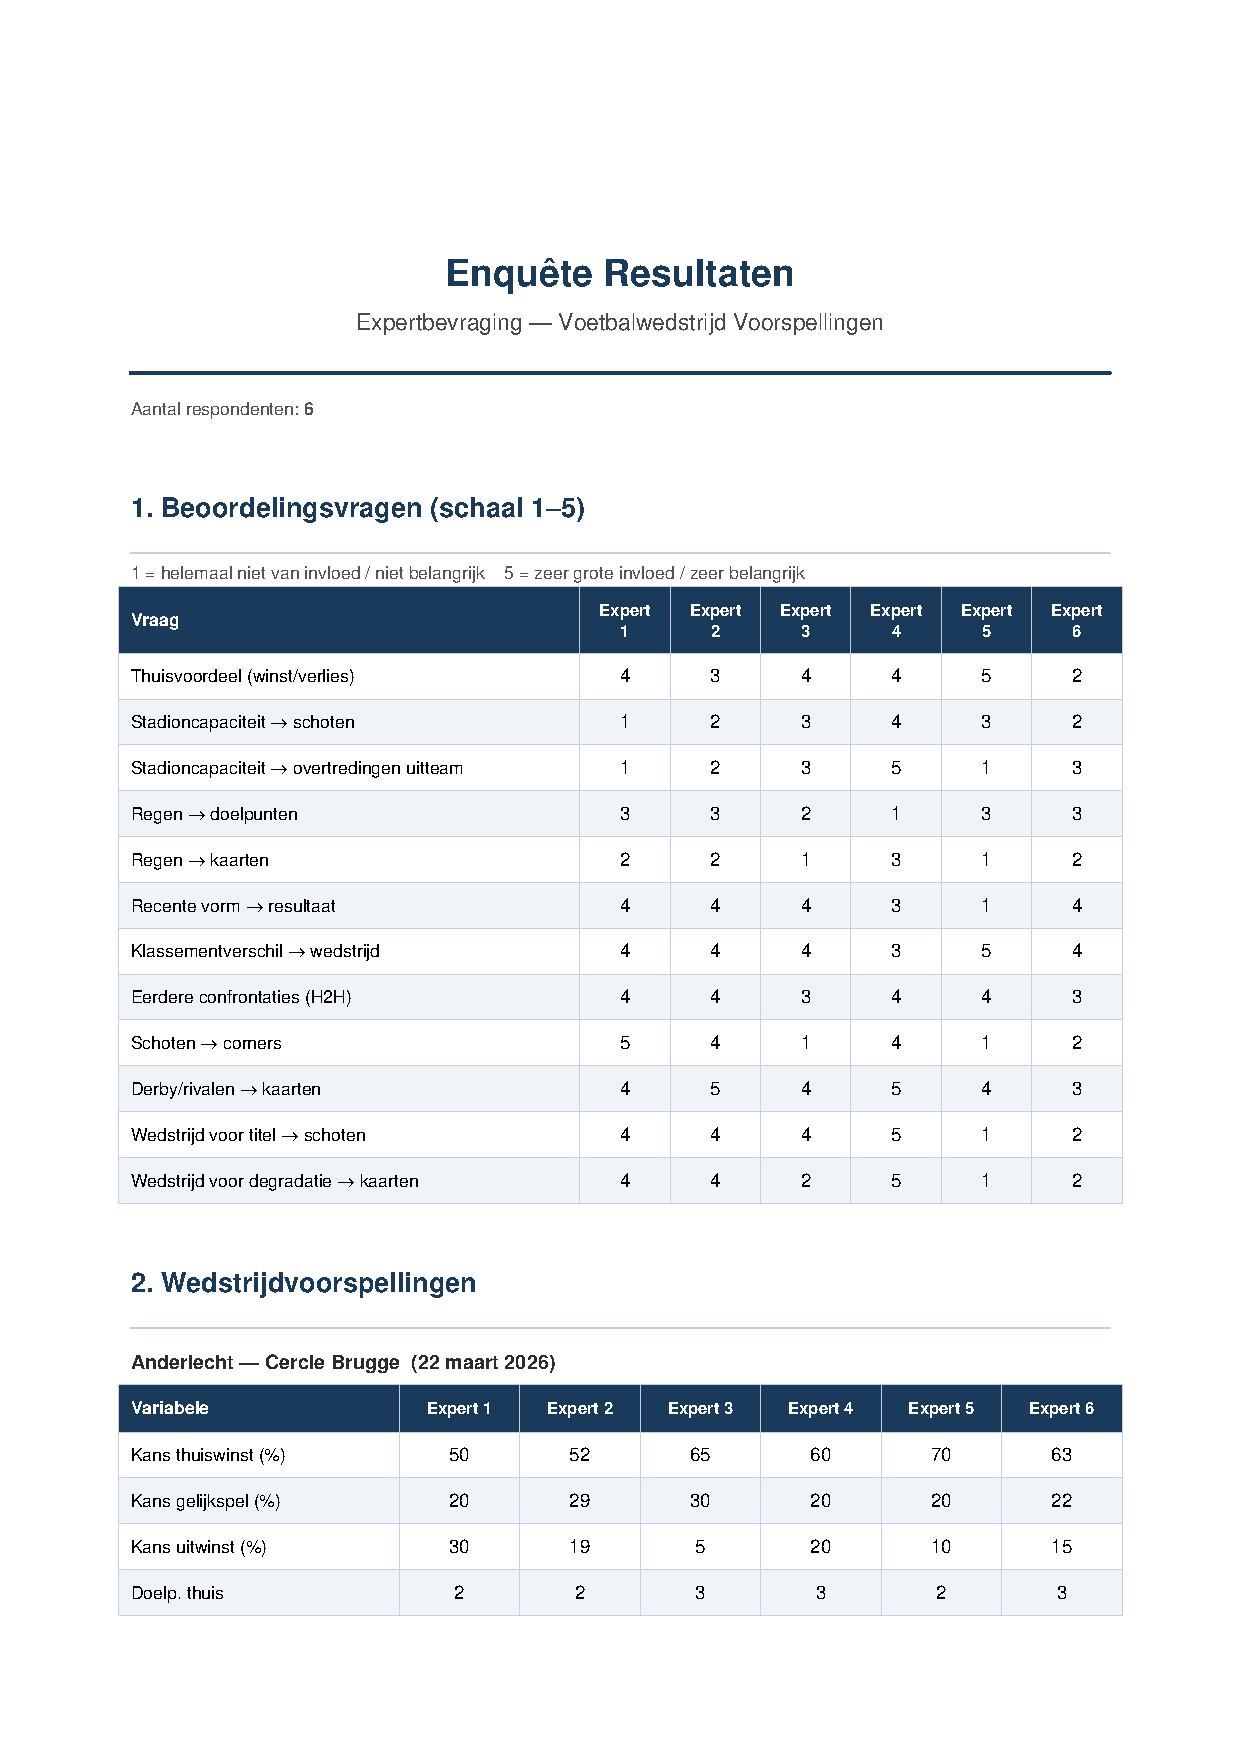
\includepdf[pages=-,pagecommand={}]{../../code/data/enquete_resultaten.pdf}

%%---------- Backmatter, referentielijst ---------------------------------------

\backmatter{}

\setlength\bibitemsep{2pt} %% Add Some space between the bibliograpy entries
\printbibliography[heading=bibintoc]

\end{document}
